\documentclass{standalone}
\usepackage{tikz}

\begin{document}
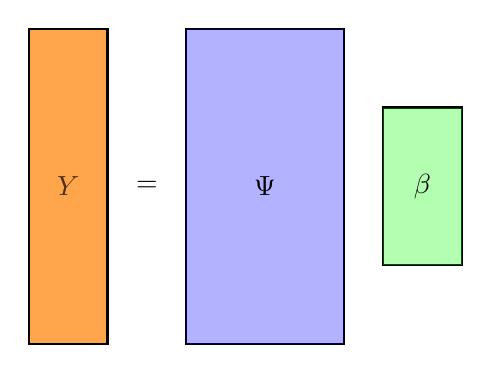
\begin{tikzpicture}
  \node(rect) at (0,0)[draw, thick, fill=orange, fill opacity=0.7, minimum width=1cm,
  minimum height=4cm]{$Y$};

  \node at (1,0) {$=$};
  \draw[thick](1.5,-2) rectangle(3.5,2);
  \fill[blue, opacity=0.3] (1.5, -2) rectangle (3.5,2);
  \node at (2.5,0) {$\Psi$};
  \draw[thick](4,1) rectangle(5,-1);
  \fill[green, opacity=0.3] (4, 1) rectangle (5, -1);
  \node at (4.5,0) {$\beta$};

\end{tikzpicture}
\end{document}
